\subsubsection{Introducción a filtros Anti Aliasing}
Un filtro \textbf{Anti Aliasing} es un filtro pasa bajos, el cual se encarga de que se cumpla el criterio de muestreo de \textbf{Nyquist}. Este postula que, para la reconstrucción exacta de una señal periódica continua en banda base, es necesaria una frecuencia de muestreo $f_s$ de un valor por lo menos 2 veces superior al ancho de banda B de la señal original. Bajo estas condiciones, para reconstruir la señal solo hace falta realizar la convolución de la muestreada con la función $sinc(B\cdot t$).

La señal original se puede expresar como:
\begin{align}
	x\left( t \right) \sim \sum_{n=-\infty}^{\infty} x\left( \frac{n}{f_s} \right) \cdot sinc \left( t-\frac{n}{f_s} \right)
\end{align}

En caso de que no se cumplan las hipótesis de Nyquist, se presenta un problema, el cual es observable utilizando el análisis de Fourier. Sea $x(t)$ una señal en tiempo continuo la cual se desea digitalizar, utilizando un muestreo ideal, se multiplica la señal por un tren periódico de deltas de período $T_s = \frac{1}{f_s}$.
\begin{align}
\delta_{T_S}(f)= \sum_{n=-\infty}^{\infty} \frac{1}{T_s} \delta(f-nf_s)
\end{align}

Así se observa la transformada de Fourier.
\begin{align}
	\mathcal{F} \{x_q(t) \} (f) =\mathcal{F} \{ \delta_{T_s} (t) \cdot x(t) \} (f)=\mathcal{F} \left\lbrace \sum_{n=-\infty}^{\infty} \delta(t-nT_s) \cdot x(nT_s)\right\rbrace (f)= X(f)\  *  \ \delta_{T_S}(f)
\end{align}

Dado que el papel de la delta en una convolución es aquel de la unidad, se nota que realizar la convolución con un tren de dicha función, es equivalente a montar el espectro de una señal sobre cada delta. El problema fundamental radica en la superposición de espectros entre una delta y la continua, como está ilustrado en la Figura (\ref{fig:alias3}). En ella se observa el caso en el cual no se cumple el teorema de Nyquist, apreciandose dicho inconveniente. En las Figuras (\ref{fig:alias4}) y (\ref{fig:aliasfin}) se termina de observar las consecuencias que esto implica.\footnote{J. G. Proakis y D. G. Manolakis, \textit{Digital signal processing}. Upper Saddle River, (Nueva Jersey): Pearson, 2014, pag 388}.

\begin{figure}[H]
	\centering
	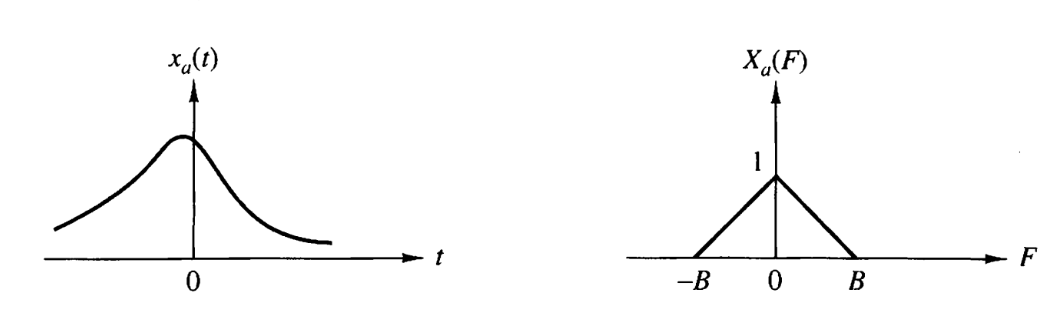
\includegraphics[width=0.8\textwidth]{ImagenesEjercicio2/aliassignal.PNG}
\caption{Señal de entrada junto a su espectro.}
	\label{fig:aliassingal}
\end{figure}
\begin{figure}[H]
	\centering
	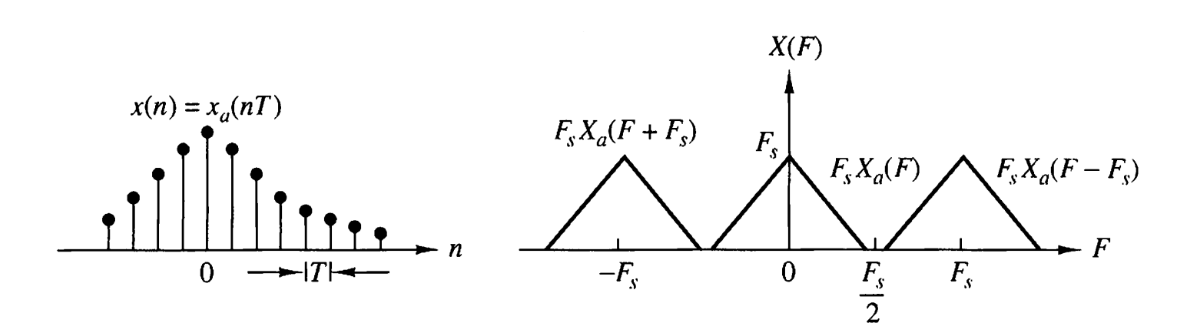
\includegraphics[width=0.8\textwidth]{ImagenesEjercicio2/aliasquatum.PNG}
\caption{Señal cuantizada junto a su espectro con $f_s > 2B$.}
	\label{fig:aliasquantum}
\end{figure}
\begin{figure}[H]
	\centering
	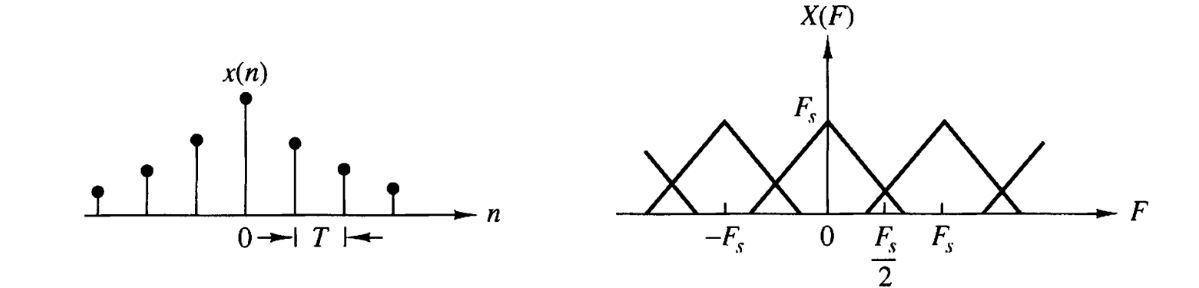
\includegraphics[width=0.8\textwidth]{ImagenesEjercicio2/alias3.PNG}
\caption{Señal cuantizada junto a su espectro con $f_s < 2B$.}
	\label{fig:alias3}
\end{figure}
\begin{figure}[H]
	\centering
	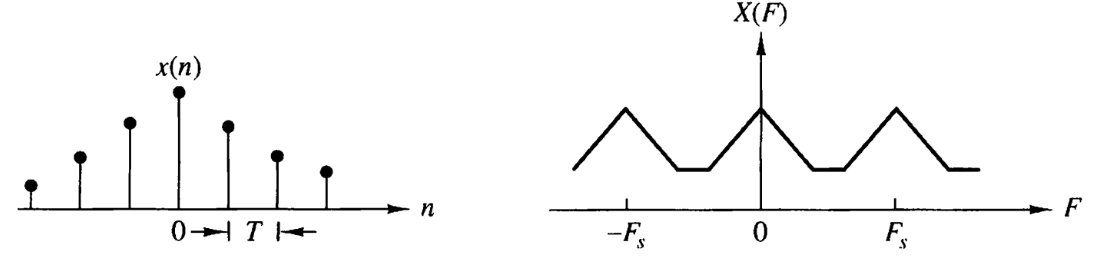
\includegraphics[width=0.8\textwidth]{ImagenesEjercicio2/alias4.PNG}
\caption{Señal cuantizada junto a su espectro resultante.}
	\label{fig:alias4}
\end{figure}
\begin{figure}[H]
	\centering
	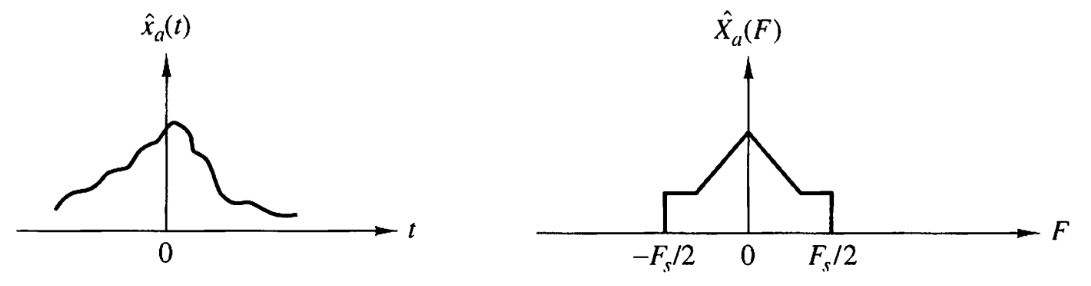
\includegraphics[width=0.8\textwidth]{ImagenesEjercicio2/aliasfin.PNG}
\caption{Señal reconstruida junto a su espectro.}
	\label{fig:aliasfin}
\end{figure}

Otro factor importante a considerar es que la frecuencia de Nyquist está definida como $2B$ únicamente para un filtro ideal. En la realidad se debe tomar una frecuencia $f_s>2B$, dado que se utiliza un filtro real.

%\begin{figure}[H]
%	\centering
%	\includegraphics[width=0.9\textwidth]{Ejercicio6/Imagenes/SalidaVsVLM35.png}
%\caption{Tensión de salida Vs. Tensión del LM35.}
%	\label{fig:vout}
%\end{figure}

\subsubsection{Introducción a filtros recuperadores}
El filtro recuperador es aquel que cumple con la tarea de recuperar la señal a partir de su espectro, dado que previo al filtro, se tiene un espectro como es observado en la Figura (\ref{fig:recuperador}). El objetivo de este es filtrar los espectros ajenos a la banda base, para obtener en el dominio temporal la señal original. Es necesario remarcar la vital importancia de recuperador, como su nombre indica.
\begin{figure}[H]
	\centering
	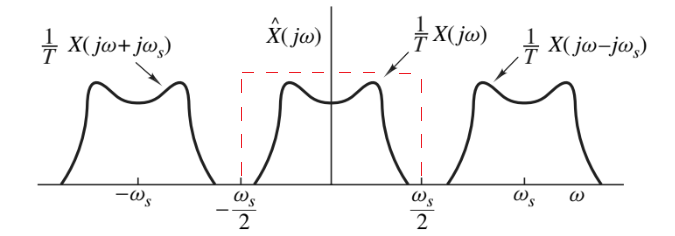
\includegraphics[width=0.8\textwidth]{ImagenesEjercicio2/recuperador.PNG}
\caption{Espectro de la señal cuantizada. En rojo el filtro recuperador ideal.}
	\label{fig:recuperador}
\end{figure}

\subsubsection{Análisis espectral}
En esta sección se procede a analizar el tipo de señales que recibe el circuito. Es así que see especifican las siguientes señales:
{\center
$X_a = cos(2 \pi f_{in} t)$ \ \ $\sim$  \ \
$X_b$: $\frac{3}{2}$ seno \  \ $\sim$ \ \
$X_c$ : Señal triangular \\
}

Para esto se utiliza como herramienta la serie de Fourier de cada una de estas señales, la cual se define como:
\begin{equation*}
x(t) = \sum_{n=-\infty}^{\infty} X_n \cdot e^{j2\pi n f_0t}
\end{equation*}
\begin{equation*}
X_n= \int_{-\frac{T}{2}}^\frac{T}{2} x(t) \cdot e^{-j2\pi n f_0t} dt
\end{equation*}

Teniendo en cuenta que tambien se puede expresar de forma trigonométrica, se puden reescribir como:
\begin{equation*}
x(t) = \sum_{n=0}^{\infty} a_n \cdot \cos(2\pi n f_0t) + b_n  \cdot \sin(2\pi n f_0t)
\end{equation*}
\begin{equation*}
a_n = \int_{-\frac{T}{2}}^\frac{T}{2} x(t) \cdot \cos(2\pi n f_0t) dt
\end{equation*}
\begin{equation*}
b_n = \int_{-\frac{T}{2}}^\frac{T}{2} x(t) \cdot \sin(2\pi n f_0t) dt 
\end{equation*}

Realizando las cuentas para cada señal, se obtiene que:
\begin{center}
$X_a$ ya es su propio desarrollo en serie.
\end{center}
\begin{equation*}
X_b = \sum_{n=0}^{\infty} \frac{12}{\pi} \cdot \frac{1}{9-4n^2} \cdot \cos(2\pi n f_0t)
\end{equation*}
\begin{equation*}
X_c = \sum_{n=1,3,5,...}^{\infty} \frac{8 \cdot (-1)^{\frac{n-1}{2}}}{\pi^2 n^2} \cdot \sin(2\pi n f_0t)
\end{equation*}

Dado que estas ultimas 2 señales cuentan con infinitos armónicos, el criterio que se decide utilizar para saber hasta cual se debe conservar consiste en tomar todos los necesarios hasta obtener una potencia del $99\%$. Es útil recordar dicha variable de una señal se encuentra en sus coeficientes de Fourier, mediante la \textbf{igualdad de Parseval}:
\begin{align}
\frac{1}{T} \cdot \int_{-\infty}^\infty |\ x(t)\ |^2 \ =\  \sum_{n=- \infty}^{\infty} |\ X_n \ |^2
\end{align}

Para las señales $X_b$ y $X_c$ se graficó la potencia en función del armónico y como queda la señal reconstruida  luego de este filtro.
\begin{figure}[H]
	\centering
	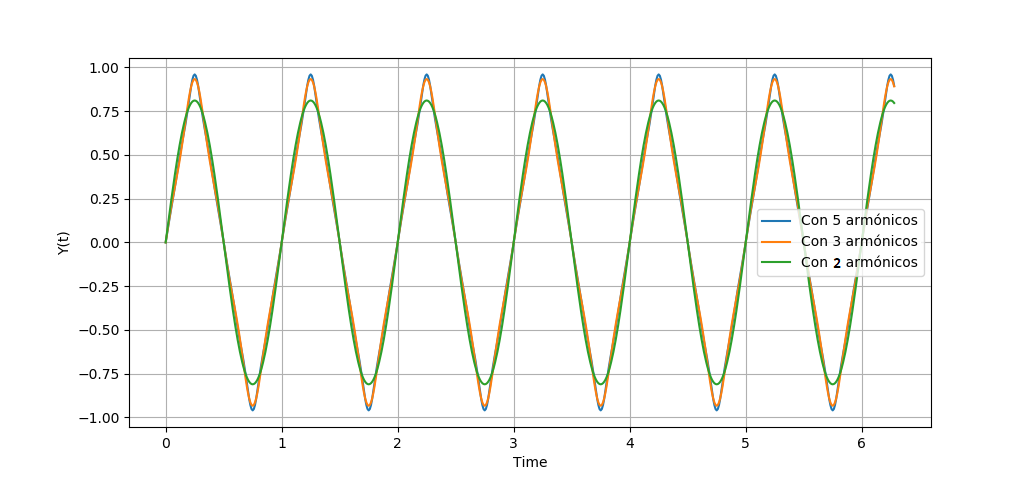
\includegraphics[width=0.85\textwidth]{ImagenesEjercicio2/10Armonicos.PNG}
	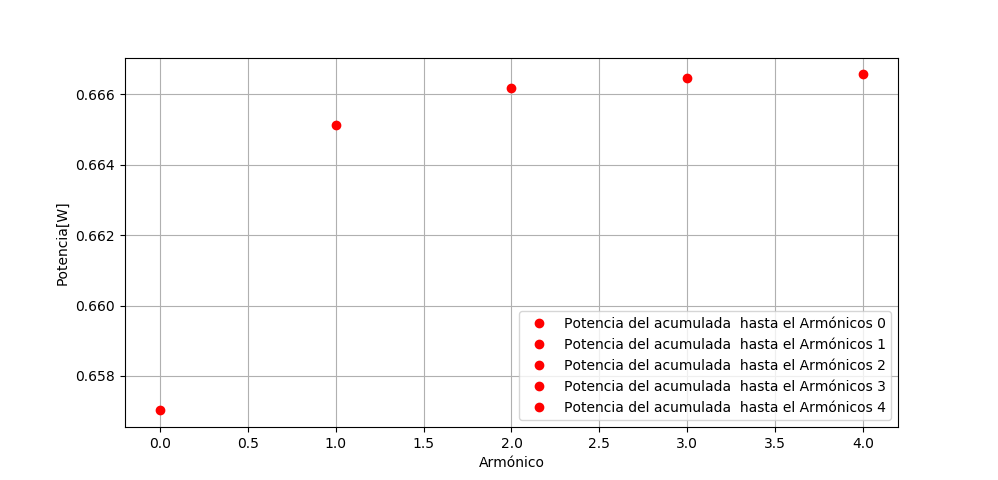
\includegraphics[width=0.85\textwidth]{ImagenesEjercicio2/4ARMONICOS.PNG}
	\caption{Señal triangular reconstruida junto a su espectro de potencias.}
	\label{fig:pottriang}
\end{figure}
\begin{figure}[H]
	\centering
	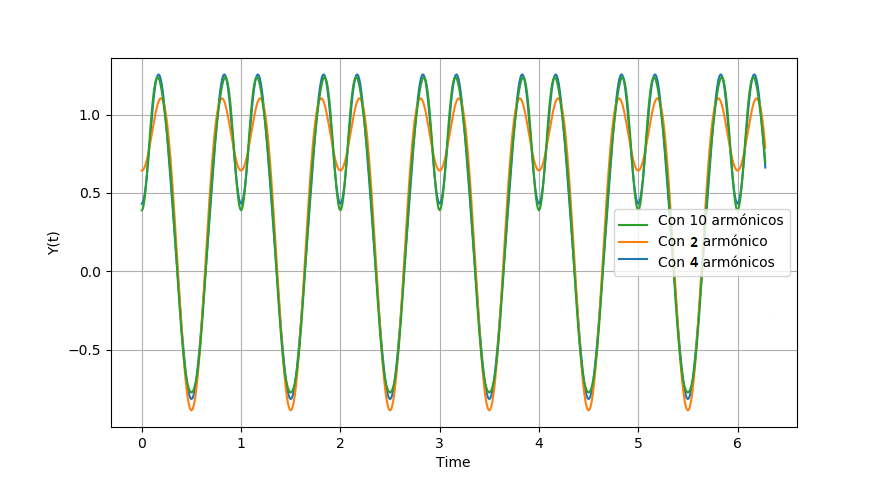
\includegraphics[width=0.85\textwidth]{ImagenesEjercicio2/sen32signal.PNG}
	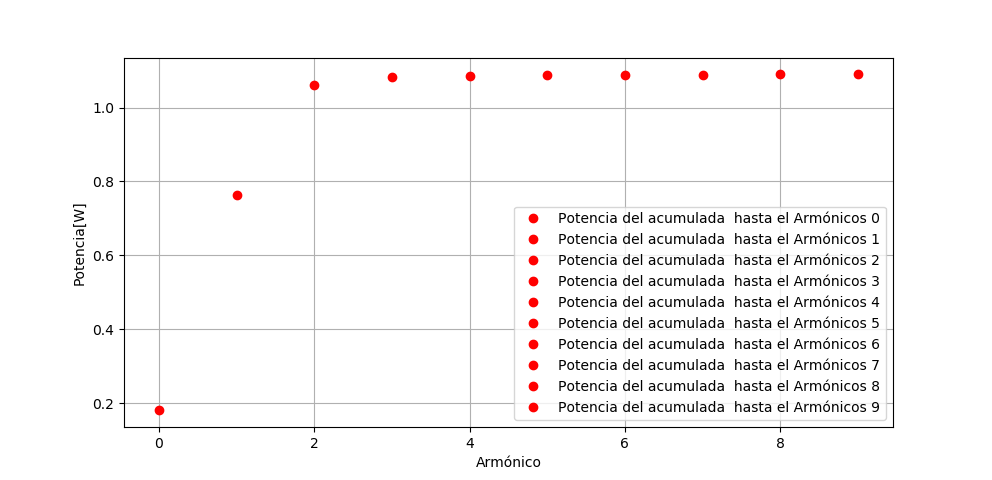
\includegraphics[width=0.85\textwidth]{ImagenesEjercicio2/sen32signalpot.PNG}
	\caption{Señal seno $\frac{3}{2}$ reconstruida junto a su espectro de potencias.}
	\label{fig:potsin}
\end{figure}

Es de interes apreciar que, para el caso de la señal triangular, tan solo con la inclusión de 2 armónicos, se obtiene una potencia superior al $98\%$. Por otro lado, se necesita incluir hasta el 3er armónico de la función  seno $\frac{3}{2}$ para obtener una potencia superior al $95\%$.

La frecuencia fundamental de estas señales es $f_0 = \frac{N}{2} = 1,5 \ kHz$, correspondiendole la del máximo armónico (es decir, el tercero) de $10.5 \ kHz$. Asimismo, es conveniente considerar la señal de AM que también es probada en el sistema, cuya máxima frecuencia es de $2,2 \cdot f_0 = 3.3 \ kHz$. Se toma $f_p= 11 \ kHz$  definiendo así la plantilla de ambos filtros:
\begin{multicols}{2}
\begin{itemize}
	\item $f_p = 11\ kHz$
	\item $f_a = 16.5 \ kHz$
	\item $A_p = 1 \ dB$
	\item $A_s = 50 \ dB$
\end{itemize}
\end{multicols}

Ya con los parámetros definidos, se procedió a elegir la aproximación a utilizar. Se descartaron las opciones de Cheby II y Cauer debido a los ceros de transmisión que estos poseen, Cheby I dado a su ripple de banda pasante, Guass y Bessel ya que su principal característica es la linealidad de la fase dejando para elegir Butterworth y Legendre. Si bien el primero tiene la mayor planicie de banda pasante, sufre de que, para cumplir plantilla, necesita un orden superior el que utiliza la segunda aproximación. Ademas, Legendre cuenta con el mayor cambio de pendiente. Por dichas razones, se decidió utilizar la aproximación de Legendre. Realizandola se obtuvo el diagrama de polos y ceros y una transferencia teórica, siendo estos los presentados acontinuación:
 \begin{figure}[H]
	\centering
	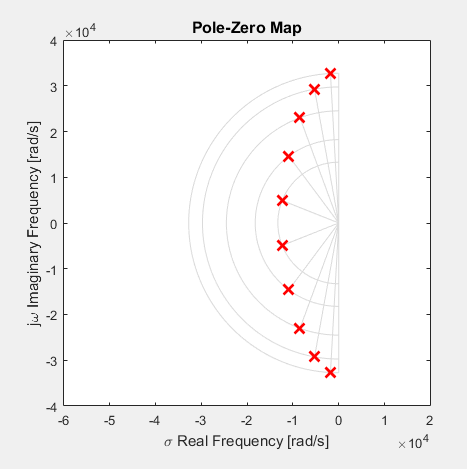
\includegraphics[width=0.65\textwidth]{ImagenesEjercicio2/polosyceros.PNG}
\caption{Diagrama de polos y ceros.}
	\label{fig:polosyceros}
\end{figure}
\begin{figure}[H]
	\centering
	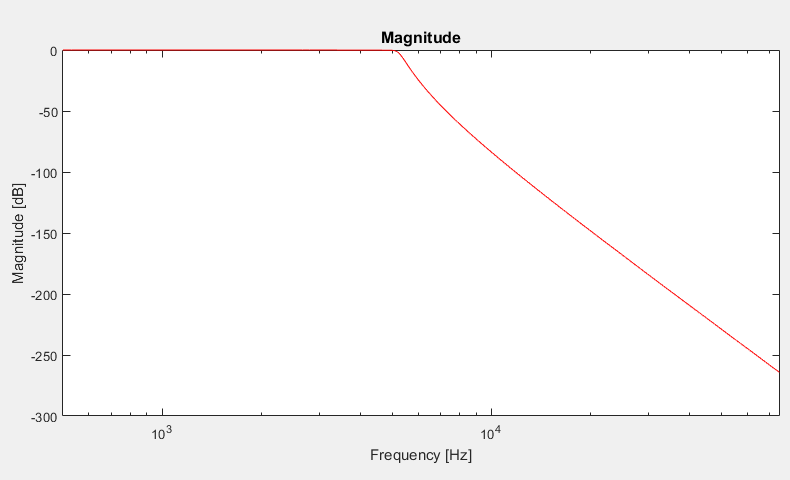
\includegraphics[width=0.8\textwidth]{ImagenesEjercicio2/atenuation.PNG}
\caption{Respuesta en frecuencia teórica.}
	\label{fig:transteorica}
\end{figure}

Sintentizando el filtro con los datos mostrado, se corresponde un filtro de orden 10, con los valores indicados en la siguiente tabla:
\begin{table}[H]
\centering
\begin{tabular}{ccc}
\hline
\textbf{Etapa} & \textbf{Frecuencia de corte [kHz]} & \textbf{Q} \\ \hline
1 & 4.5 & 0.54 \\
2 & 6.2 & 0.84 \\
3 & 8.3 & 1.45 \\
4 & 10.1 & 2.82 \\
5 & 11.2 & 9.06 \\ \hline
\end{tabular}
\caption{Frecuencias de corte y Q de las etapas del filtro deseado.}
\end{table}

La topología elegida para realizar las etapas viene dada por la \textbf{Sallen Key} pasa bajos, debido a que no se alcanzan valores altos de Q, siendo el siguiente el circuito correspondiente.
\begin{figure}[H]
\centering
	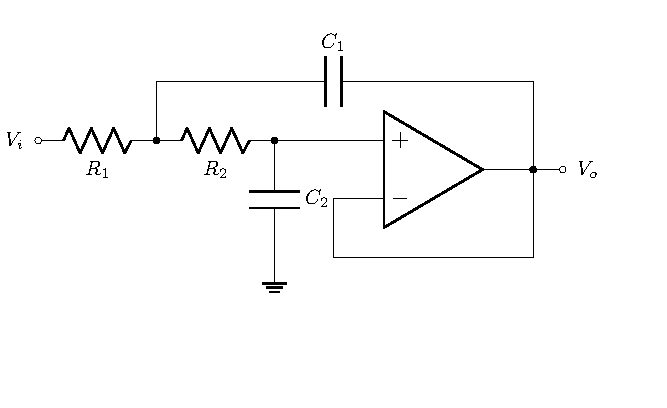
\includegraphics[width=0.7\textwidth]{ImagenesEjercicio2/SK.pdf}
	\caption{Celda Sallen Key.}
	\label{fig:SK}
\end{figure}

Luego se obtuvieron los siguientes valores para los componentes:
\begin{multicols}{2}
\begin{table}[H]
\centering
\begin{tabular}{cccc}
\hline
Componente & Valor & Valor comercial & Error \\ \hline
$R_1$ & $100 \ k\Omega$ & $100 \ k\Omega$ & $0\%$ \\
$R_2$ & $100 \ k\Omega$ & $100 \ k\Omega$ & $0\%$\\
$C_1$ & $378.6pF \ pF$ & $390 \ pF + 12 \ nF$ & $0.2\%$ \\
$C_2$ & $326.8pF \ pF$ & $330 \ pF + 33 \ nF$ & $\le0.1\%$ \\ \hline
\end{tabular}
\caption{Componentes de la etapa 1.}
\end{table}

\begin{table}[H]
\centering
\begin{tabular}{cccc}
\hline
Componente & Valor & Valor comercial & Error \\ \hline
$R_1$ & $100 \ k\Omega$ & $100 \ k\Omega$ & $0\%$ \\
$R_2$ & $100 \ k\Omega$ & $100 \ k\Omega$ & $0\%$\\
$C_1$ & $552.6 \ pF$ & $560 \ pF + 39 \ nF$ & $\le0.1\%$ \\
$C_2$ & $65.8 \ pF$ & $82 \ pF + 330 \ pF$ & $0.2\%$ \\ \hline
\end{tabular}
\caption{Componentes de la etapa 3.}
\end{table}
\begin{table}[H]
\centering
\begin{tabular}{cccc}
\hline
Componente & Valor & Valor comercial & Error \\ \hline
$R_1$ & $100 \ k\Omega$ & $100 \ k\Omega$ & $0\%$ \\
$R_2$ & $100 \ k\Omega$ & $100 \ k\Omega$ & $0\%$\\
$C_1$ & $429.1 \ pF$ & $39 \ pF // 390 \ pF$ & $0.4\%$ \\
$C_2$ & $153.3 \ pF$ & $3.3 \ pF // 150 \ pF$ & $0.1\%$ \\ \hline
\end{tabular}
\caption{Componentes de la etapa 2.}
\end{table}
\begin{table}[H]
\centering
\begin{tabular}{cccc}
\hline
Componente & Valor & Valor comercial & Error \\ \hline
$R_1$ & $100 \ k\Omega$ & $100 \ k\Omega$ & $0\%$ \\
$R_2$ & $100 \ k\Omega$ & $100 \ k\Omega$ & $0\%$\\
$C_1$ & $884.9 \ pF$ & $68pF // 820pF $ & $0.3\%$ \\
$C_2$ & $27.9 \ pF$ & $33 \ pF + 180 \ pF$ & $\le0.1\%$ \\ \hline
\end{tabular}
\caption{Componentes de la etapa 4.}
\end{table}
\end{multicols}
\begin{table}[H]
\centering
\begin{tabular}{cccc}
\hline
Componente & Valor & Valor comercial & Error \\ \hline
$R_1$ & $100 \ k\Omega$ & $100 \ k\Omega$ & $0\%$ \\
$R_2$ & $100 \ k\Omega$ & $100 \ k\Omega$ & $0\%$\\
$C_1$ & $2.6 \ nF$ & $3.3 \ nF + 12 \ nF$ & $\le0.1\%$ \\
$C_2$ & $7.9 \ pF$ & $8.2 \ pF + 220 \ pF$ & $0.3\%$ \\ \hline
\end{tabular}
\caption{Componentes de la etapa 5.}
\end{table}

Para la implementación se optó por utilizar amplificadores del tipo \href{http://www.ti.com/lit/ds/symlink/tl082.pdf}{TL084} debido a que cada integrado cuenta con 4 opamps, a su elevada impedancia de entrada y a su ancho de banda. Se simuló en \textbf{LTSpice} el filtro completo, obteniendo así la respuesta en frecuencia del mismo como se ve a continuación:
 \begin{figure}[H]
	\centering
	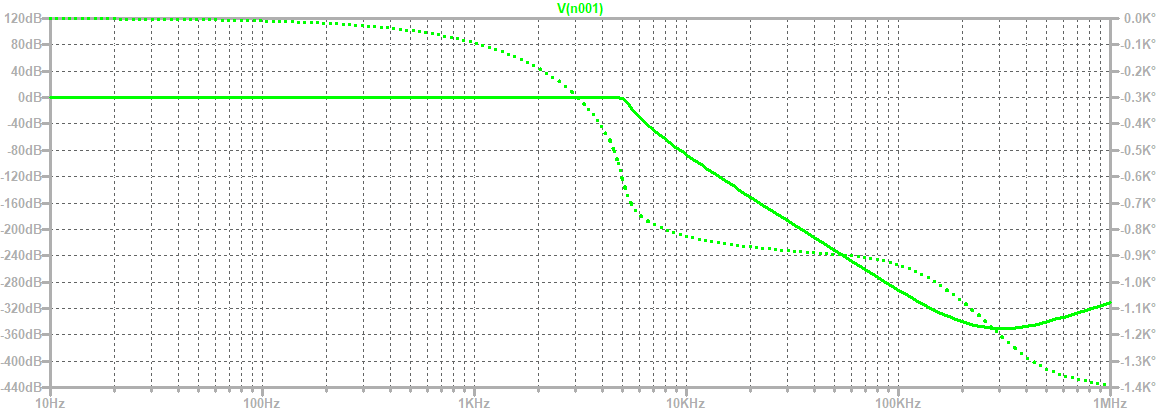
\includegraphics[width=0.8\textwidth]{ImagenesEjercicio2/spice.PNG}
\caption{Respuesta en frecuencia simulada.}
	\label{fig:transspice}
\end{figure}
A continuación se hizo un análisis de montecarlo del filtro, obteniendo una ligera desviación respecto del filtro deseado, la cual aun asi se ajusta a la plantilla con la eventual ganancia en el sobrepico.
 \begin{figure}[H]
	\centering
	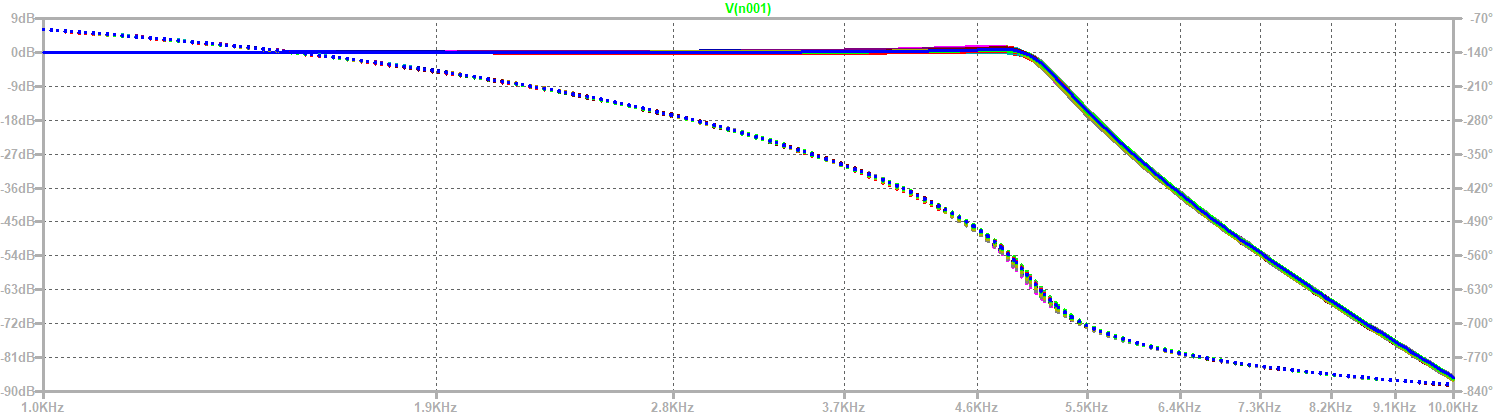
\includegraphics[width=0.8\textwidth]{ImagenesEjercicio2/montecarlo.PNG}
\caption{Montecarlo de la respuesta en frecuencia.}
	\label{fig:montecarlo}
\end{figure}
Luego, se realizó el diseño en \textbf{Altium} de la placa a realizar, obteniendo llegandose así al diseño presentado:
 \begin{figure}[H]
	\centering
	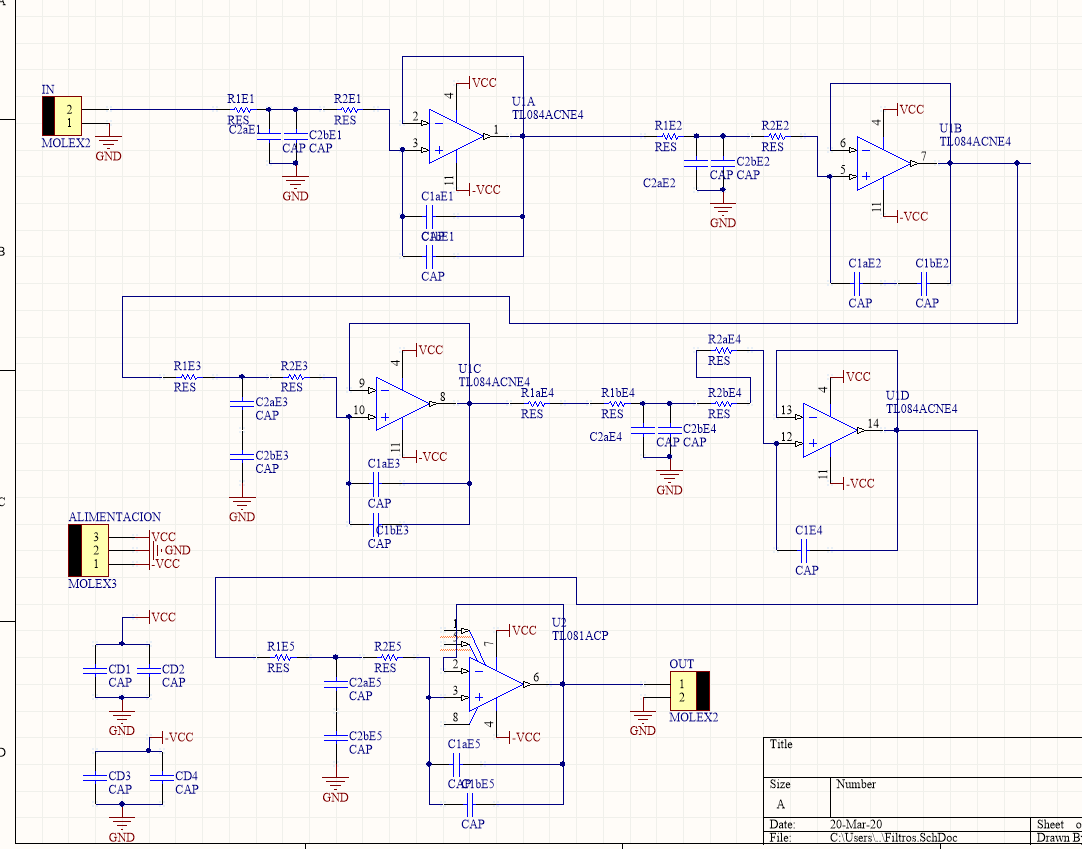
\includegraphics[width=0.6\textwidth]{ImagenesEjercicio2/altiumesq.PNG}
\caption{Esquemático Altium.}
	\label{fig:altiumesq}
\end{figure}
 \begin{figure}[H]
	\centering
	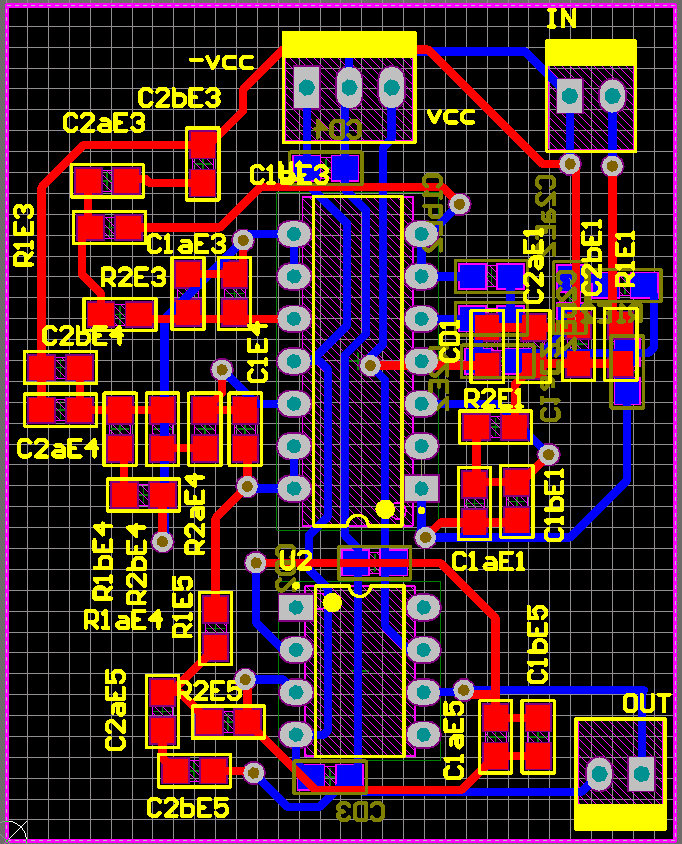
\includegraphics[width=0.6\textwidth]{ImagenesEjercicio2/altiumpcb.PNG}
\caption{PCB Altium.}
	\label{fig:altiumpcb}
\end{figure}